The gaze inference component (Section~\ref{sec:GazeInference}) estimates an initial model of the gaze behavior, which is sufficient to synthesize the entire gaze animation for the current body motion and scene. However, the animator may wish to make further edits, such as correcting errors in the actor's performance, changing the spatial layout of environment objects, and adjusting gaze to express different personality and intent. We make such edits easier to accomplish than using a traditional keyframing workflow, by relying on a model of gaze that abstracts away kinematic details of eye, head, and torso movements, and provides a set of convenient gaze editing operations. We also provide an intuitive graphical tool for performing these operations.

\subsection{Editing Operations}

Our approach allows the following editing operations. (1) The animator can edit where the character is looking by moving gaze targets or scene objects to which they are attached. The animator can also directly edit the parameters of specific gaze instances, such as (2) setting a different gaze target, (3) adjusting head and torso posture using alignment parameters, and (4) changing the timing (start and end frames). Finally, the animator can (5) add new gaze instance and (6) remove existing ones. For all these operations, the synthesis component (Section~\ref{sec:GazeSynthesis}) automatically synthesizes the gaze animation that matches the new specification.

Implementations of operations 1-3 are straightforward, since they only change specific properties of the gaze instances, while changes to the animation are effected by the synthesis component. Operations 4-6 change the timing and content of gaze instances, so we designed them to preserve the validity of the gaze sequence. Two gaze instances may not overlap, so when adding or extending a gaze instance, we either trim or remove the adjacent gaze instances. Gaze instances must have a minimal length (0.3 seconds by default), since the gaze controller requires some time to execute a gaze shift; if trimming a gaze instance would shorten it below that threshold, we remove it instead. Finally, removing gaze instances may introduce gaps into the gaze sequence, where the character's gaze is unconstrained. At the beginning of each such gap, we automatically insert a new gaze instance that realigns the gaze direction with the original motion and simultaneously blends out the gaze animation (as described in Section~\ref{sec:GazeMotionBlending}), thus ensuring smooth transition to the original motion.

\subsection{Editing Tool}

We have implemented the gaze editing operations in a plugin for the Unity game engine\footnote{http://unity3d.com/}. Most of the system functionality, including gaze inference and animation playback and layering, is implemented as Unity Editor scripts. The main synthesis components---gaze controller and IK solver---are implemented as Unity components and attached to character models in the scene.

Gaze editing operations are exposed as graphical controls integrated in the Unity Editor interface. Figure~\ref{fig:GazeEditingTool} shows the main gaze editing controls. Gaze targets are visually indicated in the scene view (1). The current sequence of gaze instances is indicated as a directed polyline connecting the gaze targets (2).  The animator can use the timeline control (3) to play or scrub along the current animation. If there is a gaze instance active at the current frame, the corresponding polyline segment is highlighted (4). Positions of the alignment handles (5) along the segments are proportional to the value of alignment parameters in the current gaze annotation (0-1 range); the animator can edit alignment values by clicking and dragging the handles. Buttons below the timeline (6) invoke gaze editing operations, such as adding a gaze instance starting at the current frame, or removing the currently active gaze instance. When the animator is satisfied with the edits they have made, they can click the Apply button (7) to synthesize the new gaze animation.

\begin{figure}
\centering
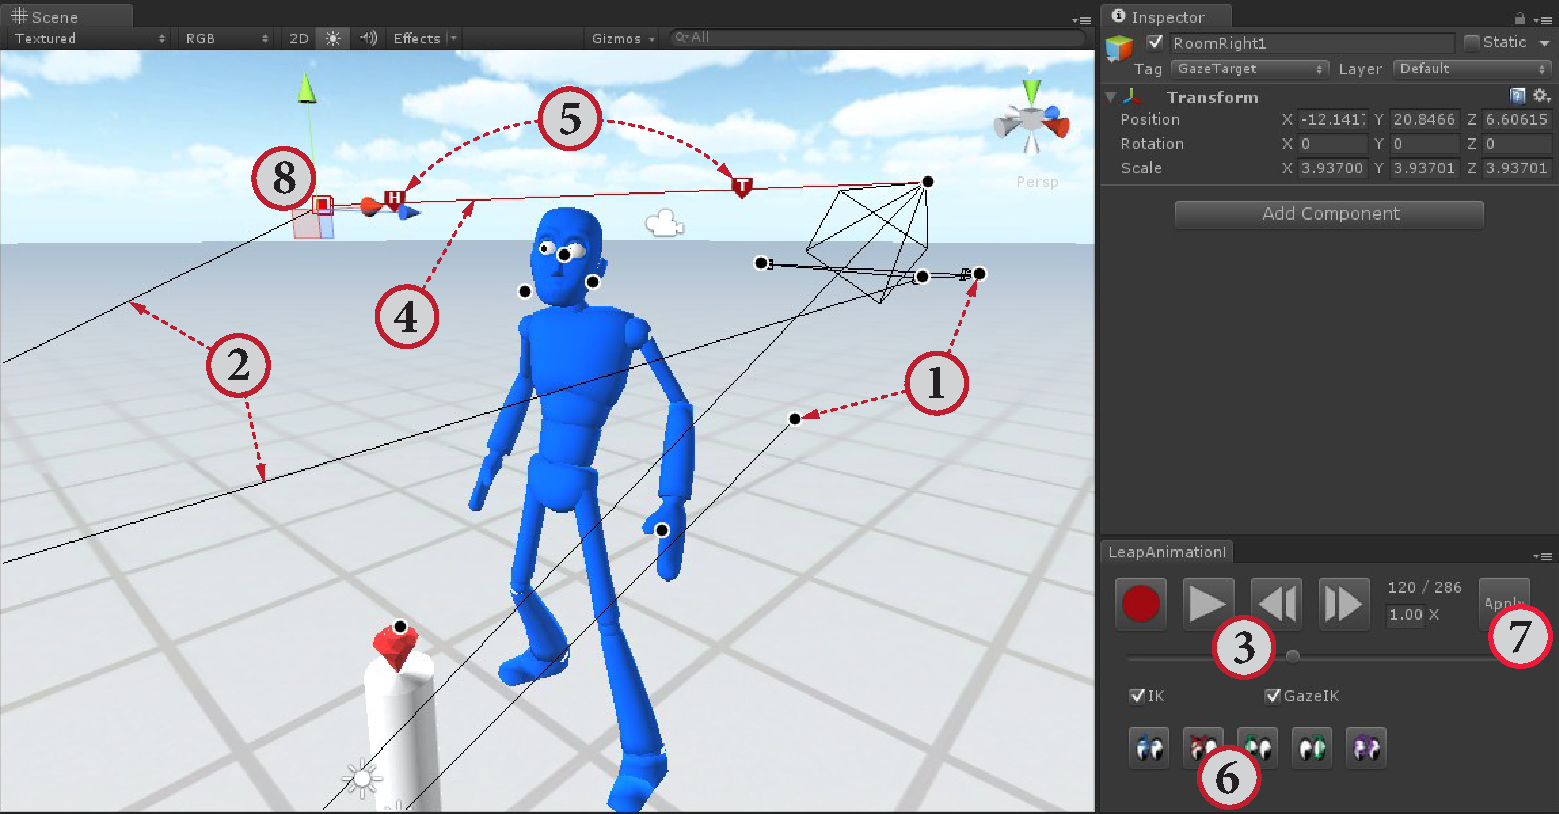
\includegraphics[width=0.48\textwidth]{Figures/GazeEditingTool.pdf}
\caption{Screenshot of the gaze editing interface: (1) gaze targets, (2) gaze sequence polyline, (3) timeline controls, (4) currently active gaze instance, (5) alignment parameter handles (H -- head alignment; T -- torso alignment), (6) gaze editing operations, (7) Apply button synthesizes the edited animation, (8) widget for moving a selected object or gaze target.}
\label{fig:GazeEditingTool}
\end{figure}
%To perform a gaze editing operation, the animator navigates to the desired position on the timeline and invokes the operation by clicking the appropriate button or using a keyboard shortcut. In the example shown in Figure~\ref{fig:GazeEditingTool}, to create a new gaze shift toward the gem starting at frame 106, the animator would use the timeline to navigate to that frame, select the gem's gaze target by clicking on it in the scene, and click the Add Gaze button.

Gaze targets are implemented as tagged, dummy objects parented to scene objects and visually indicated in the scene view (8). For example, there is a gaze target object attached to the gem in Figure~\ref{fig:GazeEditingTool}. A large object can have multiple targets attached at different locations. Spatial editing of gaze can be done either by directly selecting and moving gaze target handles or by moving the scene objects to which they are attached. The latter method allows large-scale edits---all gaze shifts toward affected targets will adapt to their new locations.

\subsection{Results}
\label{sec:GazeEditingResults}

Our gaze authoring approach can produce believable results while requiring less labor and skill than traditional methods. An experienced animator must set many keyframes to add eye movements to a body motion, while our system can add an equivalent amount of animation automatically. Manually adding a new gaze shift to an existing gaze animation requires setting multiple keyframes on each of the eye, head, and torso joints, whereas our tool can accomplish the same result in a single operation. Much of the challenge in producing high-quality animation comes from getting the timing right---each keyframe needs to be placed with great care. Our tool greatly reduces this burden---the gaze controller implements kinematics of human gaze and it automatically computes relative timings of eye, head, and torso movements that result in natural motion.
% In summary, when the objective is to get plausible gaze animation without any editing, complexity of traditional keyframing is always at least O(n) in motion length, whereas our approach is automatic and therefore O(1). When editing gaze animation, keyframing requires several times more operations than our approach and considerably more skill. 

\begin{figure}
\centering
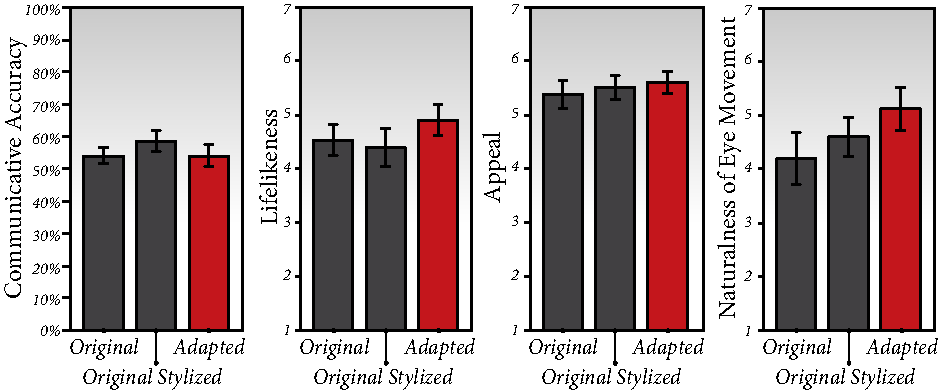
\includegraphics[width=0.46\textwidth]{Figures/Results.pdf}
\caption{Example motions generated using our system.}
\label{fig:Results}
\end{figure}

Figure~\ref{fig:Results} shows several examples of gaze animation created using approach. Each example consists of two rows of images showing two versions of the same scene. Example 1 (WalkCones) demonstrates the effects of adding inferred eye movements to a walking motion. The eye movements make the character more lifelike and anticipate changes in trajectory. Example 2 (DrinkSoda) shows a story edit where a new character is introduced and the other two characters are made to gaze at her. In Example 3 (MakeSandwich), the character making a sandwich is made to look at the camera after adding each ingredient to increase the viewer's engagement. In Example 4 (WaitForBus), we prevented the character from checking his watch by removing the corresponding gaze instance and constraining his arm. Examples 5 and 6 show how we can use gaze edits to change the character's personality. Example 5 (ChatWithFriend) contrasts two versions of a first-person conversational scene, one where the character creepily stares at the camera and another where it looks away uncomfortably. In Example 6 (HandShake), we made the character appear standoffish by having him look away during the handshake. 